\documentclass[12pt]{article}
%\documentclass{elsart}
%%\bibliographystyle{elsevier}
\usepackage{graphicx}   % need for figures
\usepackage{fancyhdr}
\topmargin -0.2in
\headheight 0.0in
\headsep 0.4in
\textheight 9.0in
\oddsidemargin -.0in
\evensidemargin -.0in
\textwidth 6.5in
\renewcommand{\baselinestretch}{1.4}
%%\usepackage{epsfig}
%%\input epsf
%%\usepackage[dvips]{color}
\usepackage{lscape}
\usepackage{longtable}
%
\def\beqn{\begin{eqnarray}}
\def\eeqn{\end{eqnarray}}
\def\beq{\begin{equation}}
\def\eeq{\end{equation}}

\pagenumbering{arabic}	

\newcommand{\la}{\langle}
\newcommand{\ra}{\rangle}
\newcommand{\zh}{z}
\newcommand{\xbj}{x_{\scriptscriptstyle B}}
%
\newcommand{\thp}{$\Theta^+$ }
\newcommand{\Thgg}{$\theta_{\gamma^*\gamma}~$}
\newcommand{\Phgg}{$\phi_{\gamma^*\gamma}~$}
\newcommand{\Epg}{$ep~\rightarrow~ep\gamma~$}
\newcommand{\Eppiz}{$ep~\rightarrow~ep\pi^0~$}
\newcommand{\Enpip}{$ep~\rightarrow~en\pi^+~$}
\newcommand{\EppiD}{$ep~\rightarrow~e\pi \Delta~$}
\newcommand{\Epeta}{$ep~\rightarrow~ep\eta~$}
\newcommand{\Epr}{$ep~\rightarrow~ep\rho~$}
\newcommand{\EpX}{$ep~\rightarrow~epX~$}
\newcommand{\EpKY}{$ep~\rightarrow~eKY~$}
\newcommand{\vEpg}{$\vec ep~\rightarrow~ep\gamma~$}
\def\gevc2{(GeV/c)$^2$}
\newcommand*{\jlab}{Jefferson Lab, Newport News, VA 23606, USA}
\newcommand*{\yerevan}{Yerevan Physics Institute, 375036 Yerevan, Armenia}
\newcommand*{\frascati}{Istituto Nazionale di Fisica Nucleare, Laboratori Nazionali di Frascati, P.O. 13, 00044 Frascati, Italy}
\newcommand*{\genova}{Istituto Nazionale di Fisica Nucleare, Sezione di Genova
 e Dipartimento di Fisica dell'Universita, 16146 Genova, Italy}
\newcommand*{\ipn}{Institut de Physique Nucleaire d'Orsay, IN2P3, BP 1, 91406 Orsay, France}
\newcommand*{\uvch}{University of Virginia, Department of Physics, Charlottesville, VA 22903, USA}
\newcommand*{\nsuva}{Norfolk State University, Norfolk VA 23504, USA}
\newcommand*{\rpi}{Rensselaer Polytechnic Institute, Department of Physics, Troy, NY 12181, USA}
\newcommand*{\moscow}{Moscow  State University, 11989 Moscow, Russia}
\newcommand*{\itep}{Institute for Theoretical and Experimental Physics, Moscow, Russia}
\newcommand*{\ucla}{University of California at Los Angeles, Department of Physics and 
Astronomy, Los Angeles, CA 90095-1547, USA}
\newcommand*{\ohio}{Ohio University, Department of Physics, Athens, OH 45701, USA}
\newcommand*{\gwu} {Center for Nuclear Studies,
The George Washington University, Washington, D.C., 20052}
\newcommand*{\jmu} {James Madison University, Harrisonburg, Virginia
22807, USA}




%
%%%%%%%%%%%%%%%%%%%%%%%%%%%%%%%%%%%%%%%%%%%%%%%%%%%%%%
%

%

\begin{document}

\thispagestyle{empty}
\begin{center}
{\Huge \bf CLAS12 DAQ and Trigger}
\end{center}
\begin{center}
{\Huge \bf Operations Manual}
\end{center}
\vspace{2cm}

\begin{center}
{\Large \bf Version 0.5}
\end{center}
\vspace{2cm}

\begin{center}
{\Large \bf Contact Person: Sergey Boyarinov}
\end{center}
\vspace{2cm}

\pagestyle{empty}

\thispagestyle{empty}

\newpage

\fancypagestyle{myheading}{%                % Redefining plain style
\fancyhf{} % clear all header and footer fields
\fancyhead[C]{\vspace{0.5cm}\line(1,0){500}\vspace{-0.5cm}}
\fancyhead[l]{\mbox{\bfseries CLAS12 DAQ and Trigger}}
\fancyhead[r]{\mbox{\bfseries Version 0.5 \date{\today}}}
%%\fancyfoot[C]{\mbox{\bfseries  \thepage }}
%%\fancyfoot[r]{\mbox{\bfseries Operations Manual}}
%%\fancyfoot[l]{\vspace{-1cm}\line(1,0){500}}
}
\renewcommand{\headrulewidth}{0pt}
\renewcommand{\footrulewidth}{0pt}
\pagestyle{myheading}

%%\input{../daq_trigger_operations_manual/main.tex}
\section{Operations Manual}

\subsection{General Information}

The {\tt CLAS12} Data Acquisition (DAQ) System is controlled by the application 
{\tt RunControl}, which can be started on any clon cluster computer running
Linux OS. Two environment variables (\$EXPID and \$SESSION) define the DAQ behavior 
and must be set before doing anything else. For all data taking operations the
`clasrun' account must be used, which will make sure that the environment is 
set correctly. For production running, \$EXPID=clasrun and \$SESSION=clasprod.

\subsection{Startup Procedures}

DAQ GUI always runs in VNC. To connect to VNC server run script {\tt'daqvnc.py connect'},
open xterminal and start runcontrol in it. Sometimes VNC server have
to be restarted. To do that, do 'ssh clasrun@clondaq6' and run scripts
{\tt'daqvnc.py stop'} and {\tt'daqvnc.py start'}. Those scripts will kill the existing
daq vncserver, if it exists, and start a new one. After VNC server is restarted, connect
to it using {\tt'daqvnc.py connect'} script.

The command {\tt runcontrol -rocs -log} will bring up the main DAQ GUI. The flag
`-rocs' will force the readout controller (ROC) screens to be included into 
the main GUI. This should always be used, unless you want to start the ROC 
screens in a separate GUI using the command `rocs'. The flag `-log'
will force the ROC screens to be logged into directory `/data/log' if
it exist. The GUI after startup is shown in Fig.~\ref{fig:runcontrol1}.

\begin{figure}[ht]
\centering
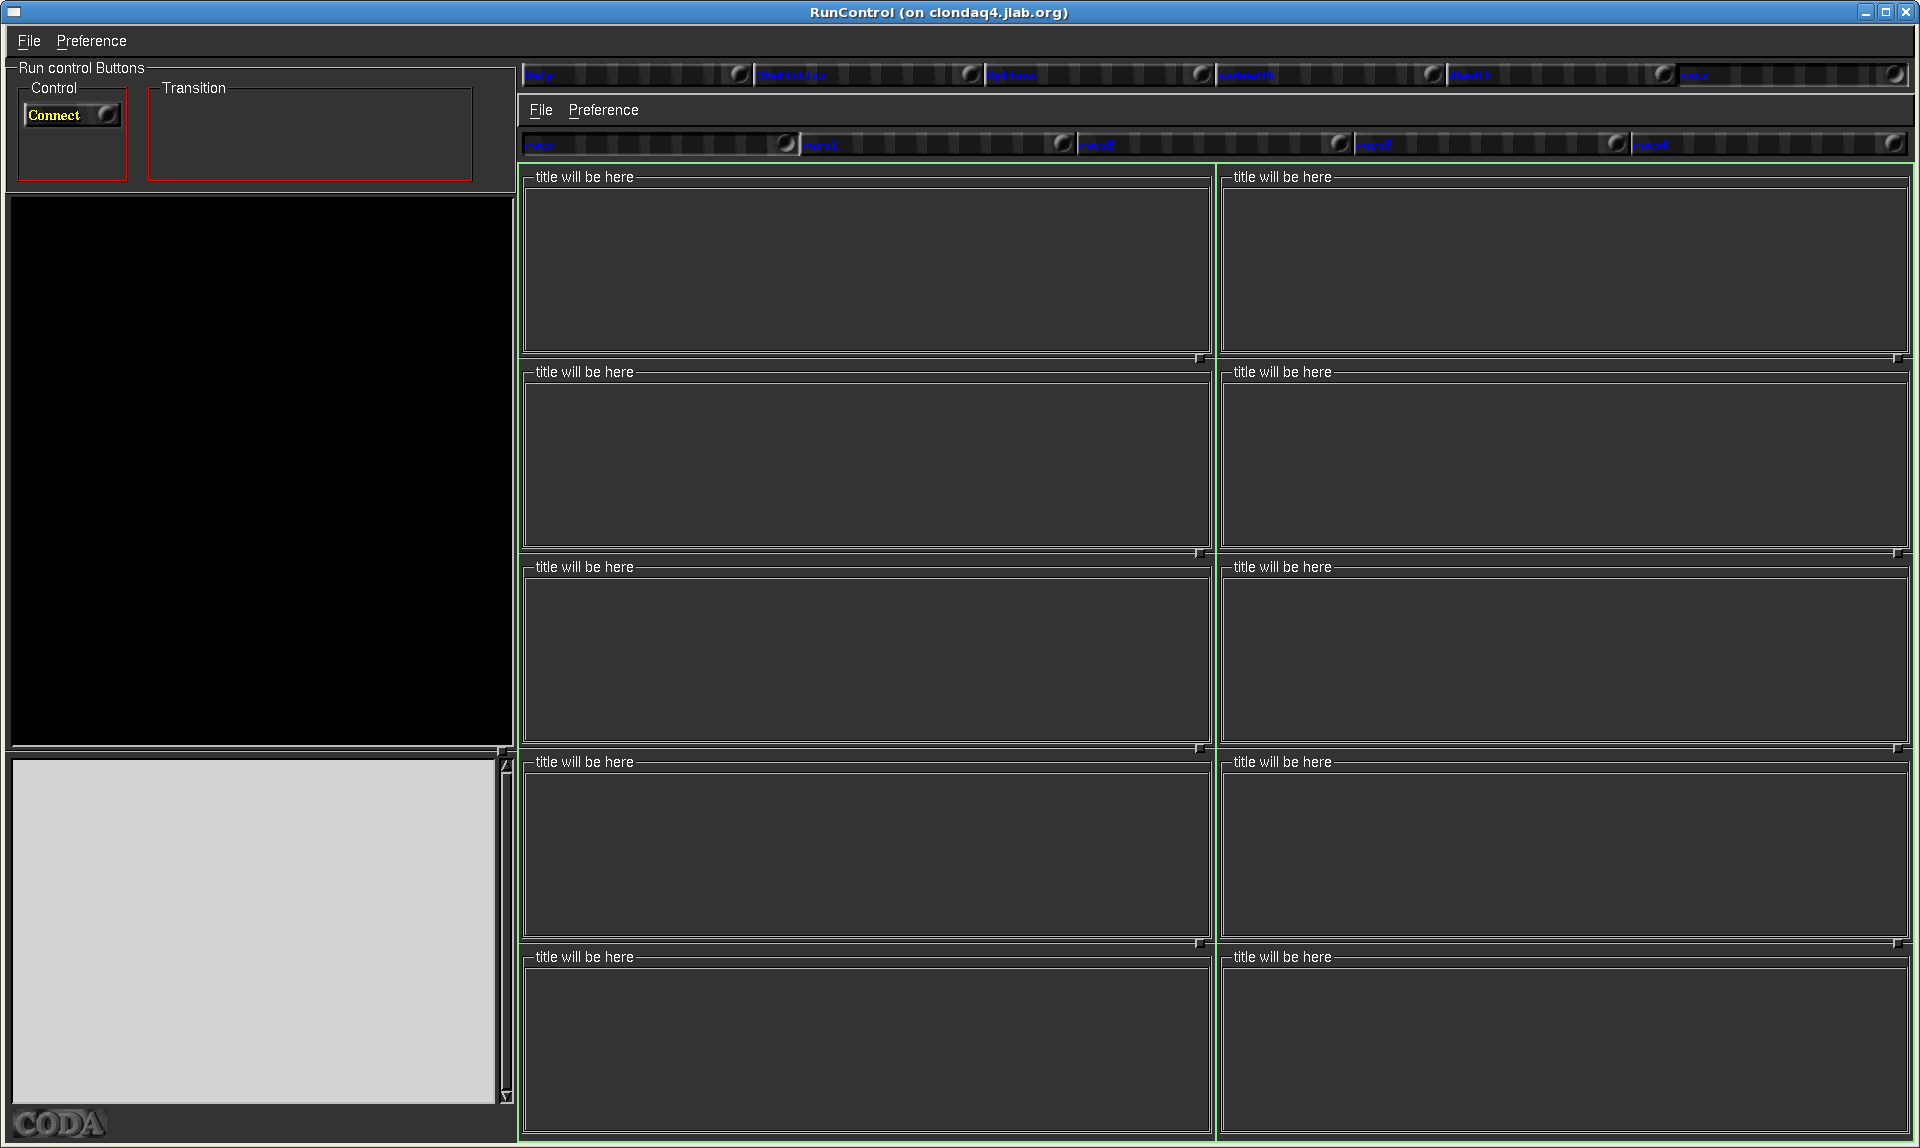
\includegraphics[width=0.9\textwidth]{runcontrol1.png}
\caption{\small{Runcontrol GUI after startup.}}
\label{fig:runcontrol1} 
\end{figure}

To proceed, click the `Connect' button. This will start the run control server
rcServer in the background or connect to the existing one (see 
Fig.~\ref{fig:runcontrol2}).

\begin{figure}[ht]
\centering
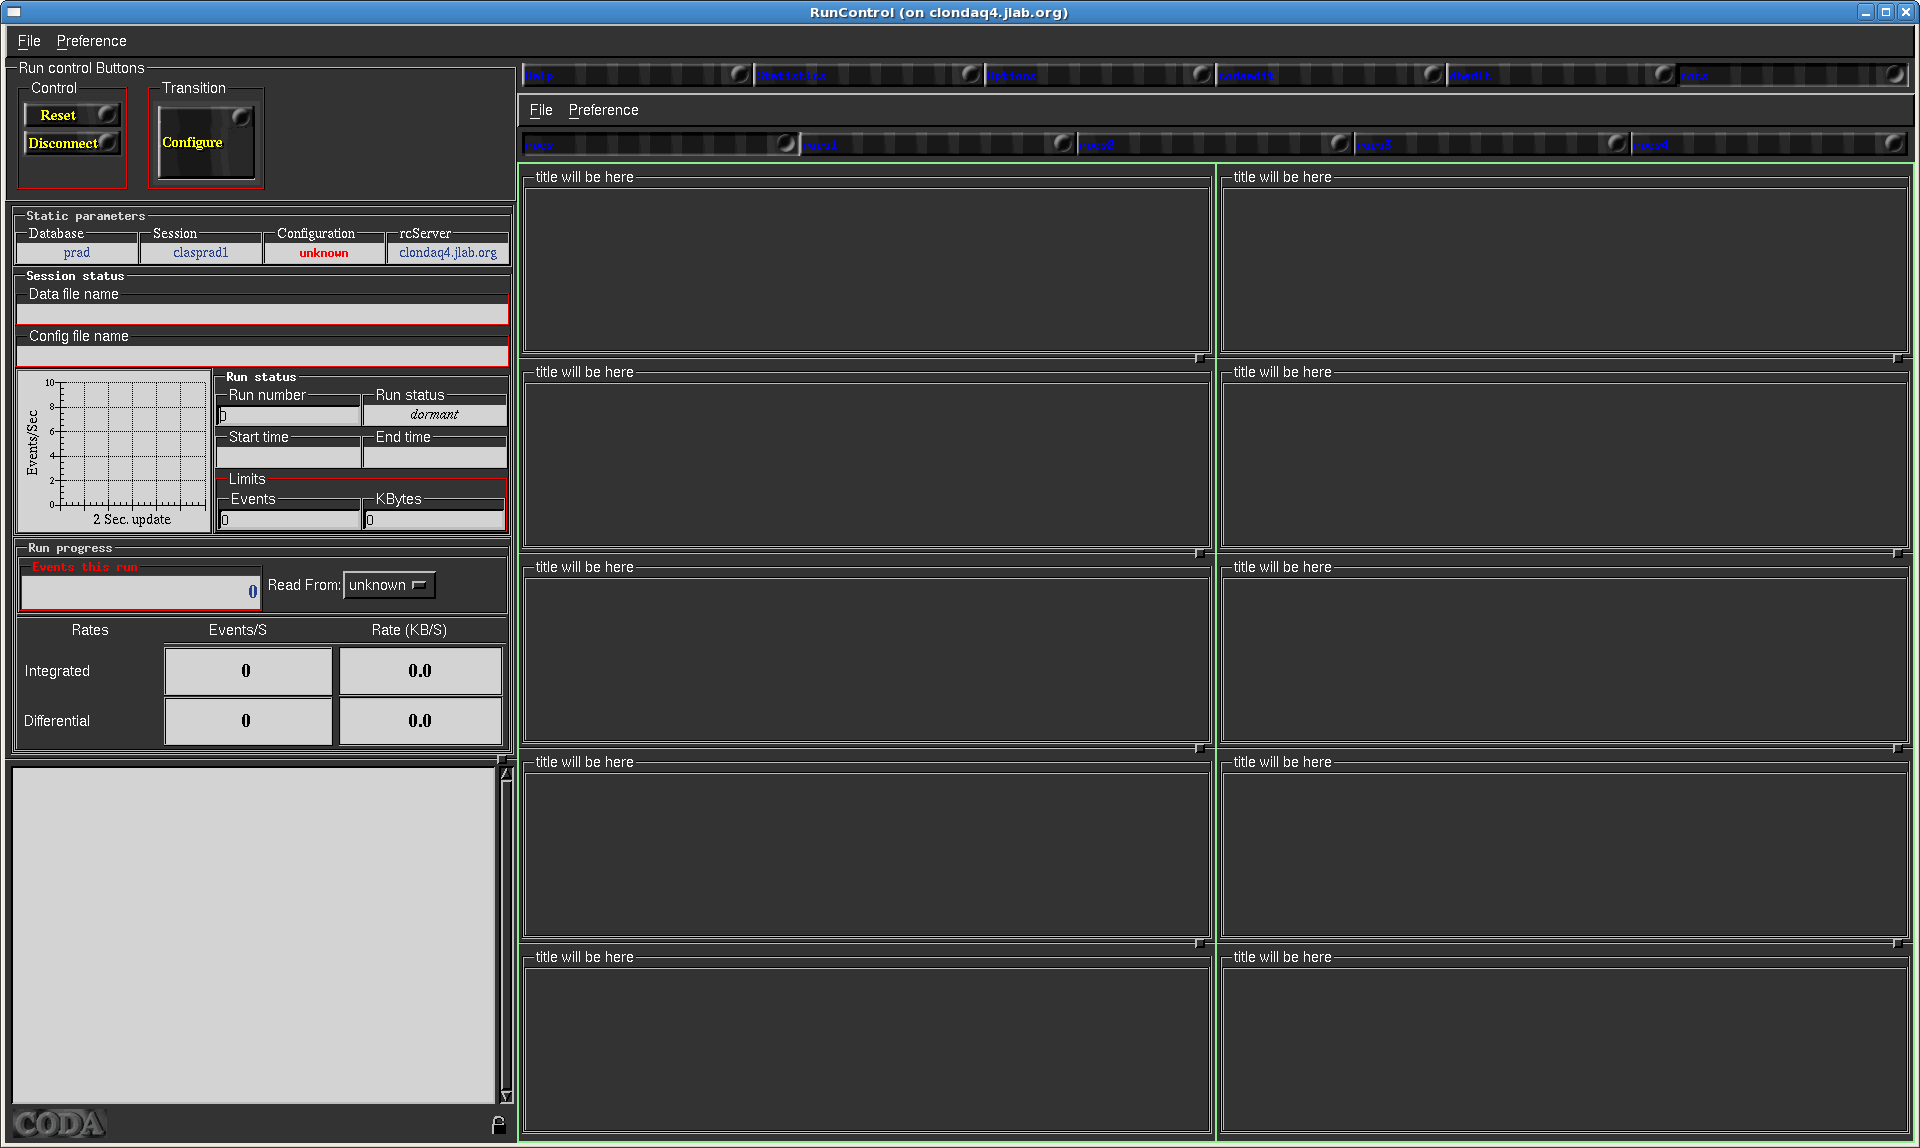
\includegraphics[width=0.9\textwidth]{runcontrol2.png}
\caption{\small{Runcontrol GUI after clicking on `Connect'.}}
\label{fig:runcontrol2} 
\end{figure}

Next, click on `Configure' and choose the DAQ configuration that you want to 
use. The DAQ configuration defines which ROCs have to be included into the
readout process. The DAQ configurations are stored in the database on the 
host defined by the environment variable \$MYSQL\_HOST. After the configuration 
is selected, the corresponding xterms will emerge on the `rocs' tab on the right 
side of the runcontrol GUI (see Fig.~\ref{fig:runcontrol3}). When all
processes are ready, 'Download' button will shows up.

\begin{figure}[ht]
\centering
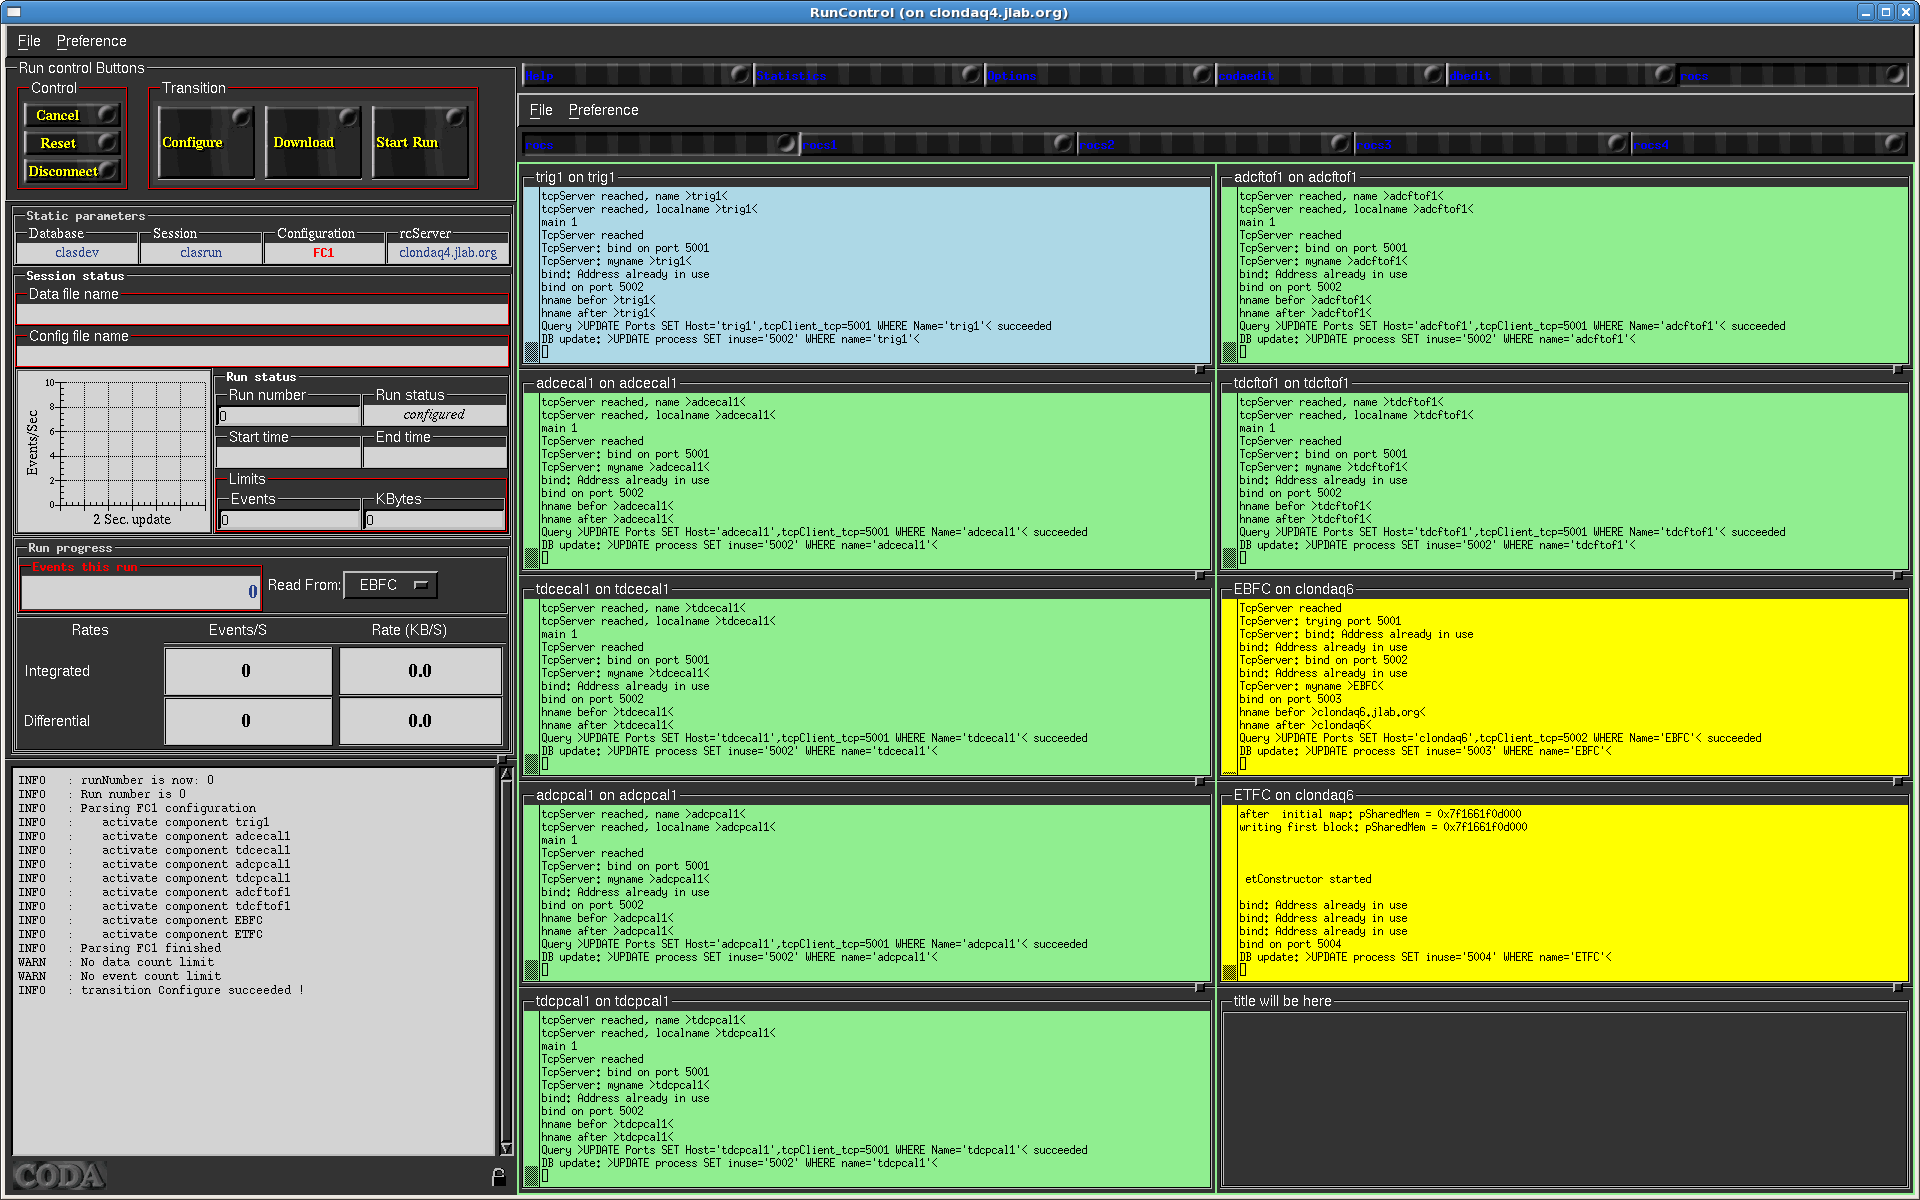
\includegraphics[width=0.9\textwidth]{runcontrol3.png}
\caption{\small{Runcontrol GUI after clicking on `Configure'.}}
\label{fig:runcontrol3} 
\end{figure}

Next, click on `Download' and choose the trigger configuration that you want to
use. The trigger configuration defines the settings to be loaded into the various
electronic modules, both trigger- and DAQ-related. The trigger configuration files 
are located in the \$CLON\_PARMS/trigger directory and its subdirectories (see 
Fig.~\ref{fig:runcontrol4}).

\begin{figure}[ht]
\centering
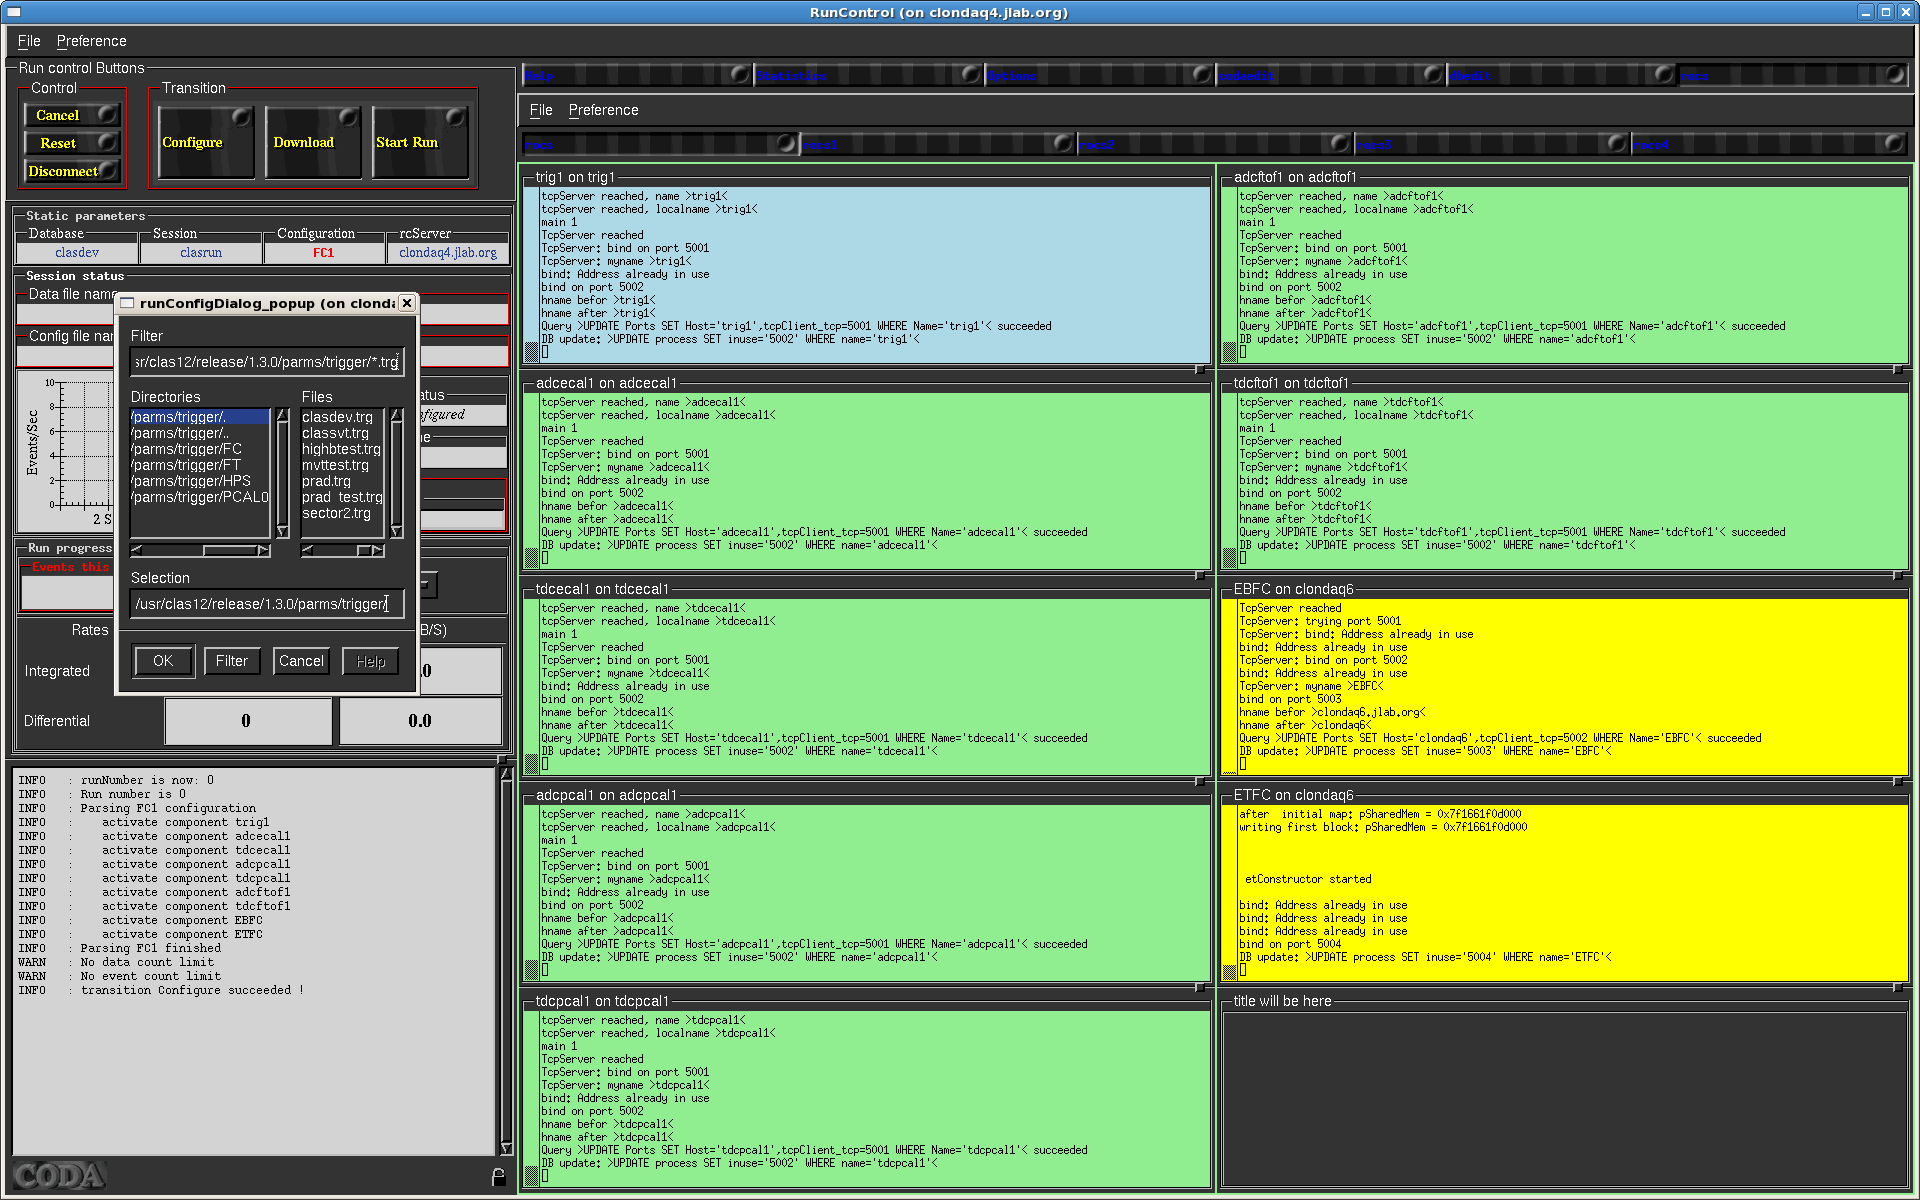
\includegraphics[width=0.9\textwidth]{runcontrol4.png}
\caption{\small{Runcontrol GUI after clicking on `Download'.}}
\label{fig:runcontrol4} 
\end{figure}

Finally, click on `Prestart' and `Go' to start a run and click `End'
to end it, and then click `Abort'. Proceed with the cycle
`Download'-`Prestart'-`Go'-`End'-`Abort' to take more runs.

%%If you want to change the trigger configuration, click on `Abort' and start
%%from `Download'.

If the DAQ has crashed, click `Abort' and `Reset' and start from `Download'.

If you want to change the DAQ configuration, click `Abort' and `Reset' and
start from `Configure'.

To exit DAQ completely, click on the `File' menu on the runcontrol GUI and
choose `Exit'.

\subsection{DAQ and Trigger Configuration Files}

The DAQ and Trigger systems are controlled by configuration files stored in
subdirectories of the \$CLON\_PARMS directory. Every DAQ module has a
designated subdirectory, for example, the configuration files for the JLab 
FADC250 modules are stored in the subdirectory `fadc250', the files for the 
CAEN TDC1190/1290 modules are stored in the subdirectory `tdc1190', and so on. 
During the `Download' transition, the DAQ will load the configuration files 
according to the following rule: if the file `XXX'.cnf exist (where XXX is the 
ROC IP name), it will be loaded, otherwise the file `\$EXPID'.cnf will be loaded. 
After that, the configuration file from the `trigger' subdirectory (chosen in the
`Download' transition using the popup GUI) will be loaded, overwriting previously 
loaded settings if necessary.



\clearpage



\end{document}
























